\documentclass[oneside,10pt]{book}

\usepackage{cdtBook}
\usepackage{usecases}

\title{Análisis}
\subtitle{}
\author{Fernández Quiñones Isaac}
\organization{Escuela Superior de Cómputo, IPN}

%%%%%%%%%%%%%%%%%%%%%%%%%%%%%%%%%%%%%%%%%%%%%%%%%%%%%%%%%%%%%%%%
\begin{document}

\maketitle
\thispagestyle{empty}

\frontmatter
\tableofcontents

\mainmatter

%=========================================================
\chapter{Introducción}

\cfinput{Introduccion}

%=========================================================
\chapter{Descripción del módulo de Torneos}

\cfinput{Descripcion}

%=========================================================
\chapter{Modelo de Negocios}

\cfinput{reglas}

%=========================================================
\chapter{Modelo de Casos de Uso}

\begin{figure}[htbp!]
		\centering
			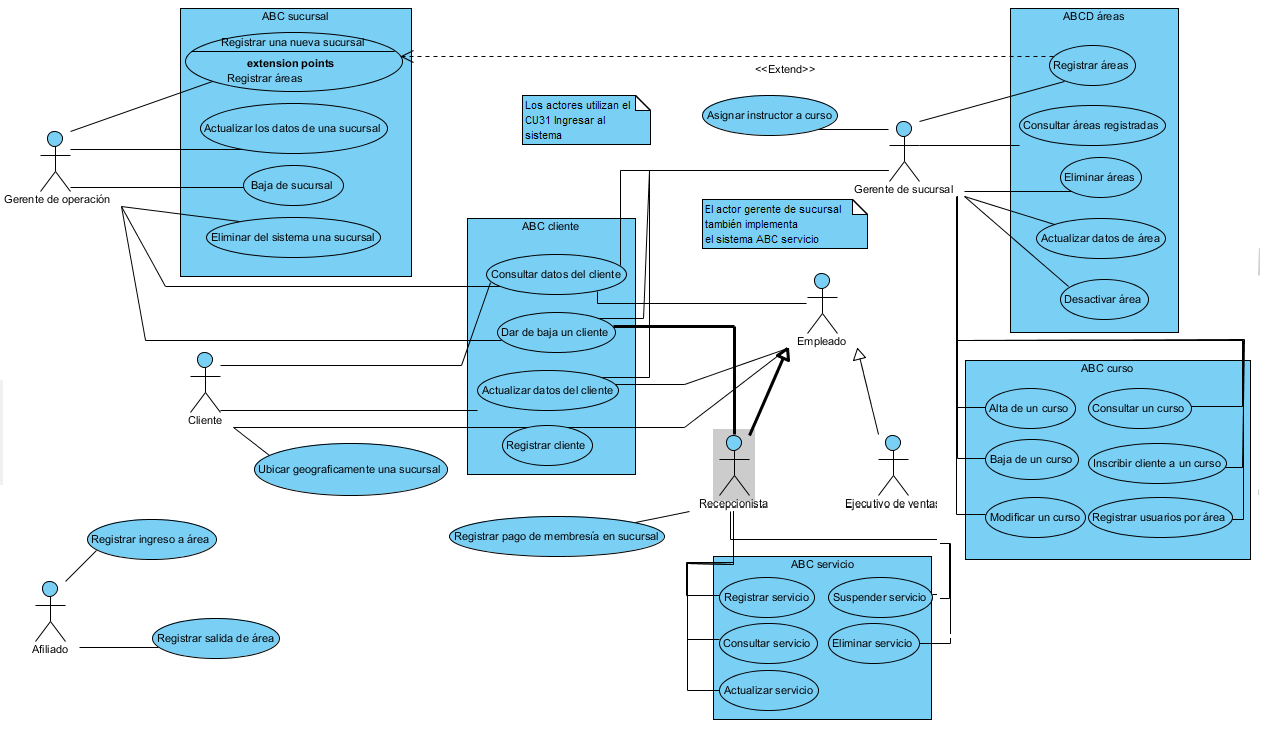
\includegraphics[width=1.2\textwidth]{images/CasosDeUso}
		\caption{Diagrama de Casos de Uso del sistema.}
	\end{figure}
	
\cfinput{cu/cu23}

%%=========================================================
\chapter{Modelo de la Interacción}

{\color{UCInterfaceColor} 
	Esta sección se queda deliberadamente en blanco debido a que el diseño de las interfaces dependerá de la plataforma a utilizar por cada equipo.\\	
}

\cfinput{Pantallas/IU23}


%=========================================================
\chapter{Actores}

\cfinput{Actores}
	
\end{document}
